\chapter{Genética del desarrollo y evolución de la forma}\label{ch:b3:developmental-genetics}

El huevo de una mosca del vinagre mide medio milímetro, y en las tres
horas que siguen a la fecundación, antes de que se haya formado una
sola membrana celular entre sus seis mil núcleos, decide qué extremo
será la cabeza y cuál la cola, dónde caerá cada uno de catorce
segmentos y cuáles de ellos llevarán patas, alas o antenas. Lo hace con
unas pocas docenas de genes, encendidos en una jerarquía de bandas cada
vez más finas, cada banda leída a partir de las concentraciones de los
productos de las bandas anteriores. En 1980, dos científicos jóvenes de
Heidelberg cribaron miles de moscas mutantes en busca de larvas con
partes ausentes o duplicadas, y hallaron toda la jerarquía: genes cuya
pérdida suprime un bloque de segmentos, genes cuya pérdida suprime un
segmento sí y otro no, genes cuya pérdida vuelve del revés cada
segmento. El trabajo de ese mismo año sobre un gen que convierte el
tercer segmento de una mosca en una copia del segundo ---y le da cuatro
alas, como tenían sus antepasados--- abrió un conjunto de genes
maestros que, se vio, están en el mismo orden a lo largo de los
cromosomas de un ratón y de un ser humano, y hacen el mismo trabajo.
Este capítulo trata de cómo un embrión calcula su propia geometría, de
cómo unos pocos cientos de genes reguladores construyen todo cuerpo
animal y de cómo cambiar cuándo y dónde actúan ha producido la
diversidad de la forma animal.

\section{Las coordenadas de la mosca}

\begin{definition}[La jerarquía de la segmentación]\label{def:b3:developmental-genetics:hierarchy}
\index{gen de efecto materno}\index{gen gap}\index{gen de regla par}\index{gen de polaridad segmentaria}\index{blastodermo sincitial}
El embrión de \emph{Drosophila} se desarrolla durante sus trece
primeras divisiones nucleares como un \emph{blastodermo sincitial}, una
sola célula cuyos núcleos comparten un citoplasma, de modo que las
proteínas difunden libremente desde donde se fabrican. Cuatro
gradientes puestos por las células de la madre fijan los ejes: el ARNm
de \emph{bicoid} queda amarrado al polo anterior y su proteína difunde
hacia atrás y forma un gradiente exponencial de la cabeza a la cola; el
ARNm de \emph{nanos} en el polo posterior hace el gradiente en espejo;
los ARNm de \emph{hunchback} y \emph{caudal} son uniformes, pero la
proteína Bicoid reprime la traducción de \emph{caudal} y Nanos reprime
la de \emph{hunchback}, de modo que sus proteínas también forman
gradientes. Estos productos de \emph{efecto materno}, cuyo fenotipo
mutante depende del genotipo de la madre y no del embrión, encienden
los \emph{genes gap} (\emph{hunchback}, \emph{Krüppel},
\emph{knirps}, \emph{giant}) en bandas anchas, cada una de las cuales
responde a un intervalo de concentración de Bicoid y reprime a sus
vecinas; las proteínas gap, en combinación, encienden los \emph{genes
de regla par} (\emph{even-skipped}, \emph{fushi tarazu}, \emph{hairy})
en siete bandas cada uno, alternadas; y las proteínas de regla par
encienden los \emph{genes de polaridad segmentaria}
(\emph{engrailed}, \emph{wingless}, \emph{hedgehog}) en catorce bandas,
una por segmento, que fijan el frente y la espalda de cada segmento y
se mantienen, una vez formadas las células, por señalización entre
ellas. Tres horas, cuatro pisos, de un solo gradiente a catorce
segmentos ---y los nombres de los mutantes recuerdan el cribado:
\emph{hunchback} carece de tórax; \emph{Krüppel} (``tullido''), de la
parte media; \emph{fushi tarazu} (``no bastantes segmentos''), de un
segmento de cada dos; \emph{hedgehog} tiene un césped de cerdas.
\end{definition}

\begin{omfigure}
\begin{tikzpicture}[every node/.style={font=\scriptsize}, >=stealth]
  \foreach \y/\lab/\n in {0/{materno: gradiente de Bicoid}/1, -1.3/{genes gap: 4 bandas anchas}/2, -2.6/{genes de regla par: 7 bandas}/3, -3.9/{polaridad segmentaria: 14 bandas}/4} {
    \draw[thick, gray!60] (0,\y) ellipse (3.6 and 0.5);
    \node[left, align=right] at (-3.8,\y) {\lab};
  }
  % bicoid gradient shading
  \begin{scope}
    \clip (0,0) ellipse (3.6 and 0.5);
    \shade[left color=omDef!80, right color=omDef!2] (-3.6,-0.5) rectangle (3.6,0.5);
  \end{scope}
  \node[right, font=\tiny] at (3.7,0) {anterior alto};
  % gap bands
  \begin{scope}
    \clip (0,-1.3) ellipse (3.6 and 0.5);
    \fill[omDef!50] (-3.4,-1.8) rectangle (-1.6,-0.8); \fill[omThm!40] (-1.4,-1.8) rectangle (0.2,-0.8); \fill[omMeth!40] (0.4,-1.8) rectangle (1.7,-0.8); \fill[omProp!45] (1.9,-1.8) rectangle (3.4,-0.8);
  \end{scope}
  \node[font=\tiny] at (-2.5,-1.3) {\emph{hb}}; \node[font=\tiny] at (-0.6,-1.3) {\emph{Kr}}; \node[font=\tiny] at (1.05,-1.3) {\emph{kni}}; \node[font=\tiny] at (2.65,-1.3) {\emph{gt}};
  % pair-rule stripes
  \begin{scope}
    \clip (0,-2.6) ellipse (3.6 and 0.5);
    \foreach \i in {0,...,6} { \fill[omThm!50] ({-3.1+\i*0.9},-3.1) rectangle ({-2.75+\i*0.9},-2.1); }
  \end{scope}
  \node[right, font=\tiny] at (3.7,-2.6) {\emph{eve}, un segmento de cada dos};
  % segment polarity stripes
  \begin{scope}
    \clip (0,-3.9) ellipse (3.6 and 0.5);
    \foreach \i in {0,...,13} { \fill[omProp!60] ({-3.25+\i*0.47},-4.4) rectangle ({-3.1+\i*0.47},-3.4); }
  \end{scope}
  \node[right, font=\tiny] at (3.7,-3.9) {\emph{en}: una por segmento};
  \foreach \y in {-0.55,-1.85,-3.15} { \draw[->, thick] (0,\y) -- (0,\y-0.2); }
  \node[below, align=center, font=\tiny] at (0,-4.5) {cada piso lee las concentraciones del piso de encima;\\tres horas desde un solo gradiente hasta catorce segmentos};
\end{tikzpicture}

{\small La jerarquía de la segmentación. Un gradiente materno se lee
como cuatro bandas de \omterm{def:b3:developmental-genetics:hierarchy}{genes gap}; las proteínas gap, en combinación,
como siete bandas de regla par; estas, como catorce bandas de polaridad
segmentaria. Cada banda es un límite trazado allí donde una
concentración cruza un umbral.}
\end{omfigure}

\begin{theorem}[Un gradiente de morfógeno a partir de síntesis, difusión y degradación]\label{thm:b3:developmental-genetics:gradient}
\index{morfógeno}\index{información posicional}\index{modelo de la bandera francesa}\index{longitud de decaimiento}
Una proteína fabricada en un extremo de un tejido a un ritmo $J$ (por
unidad de área), que difunde con coeficiente $D$ y se degrada con
constante de velocidad $k$, alcanza un estado estacionario en el que su
concentración a lo largo del eje $x$ cumple
\[
D\,\frac{\mathrm{d}^{2}c}{\mathrm{d}x^{2}} - k\,c = 0,
\qquad c(x) = c_{0}\,\mathrm{e}^{-x/\lambda}, \qquad \lambda = \sqrt{D/k},
\quad c_{0} = \frac{J}{\sqrt{Dk}} .
\]
La \emph{\omterm{thm:b3:developmental-genetics:gradient}{longitud de decaimiento}} $\lambda$ fija el alcance del
gradiente; una célula lee su posición comparando $c$ con unos umbrales
---la \emph{bandera francesa} de Wolpert (1969): por encima de $T_{1}$,
azul; entre $T_{1}$ y $T_{2}$, blanco; por debajo, rojo--- y el límite
del umbral $T$ queda en $x_{T} = \lambda\ln(c_{0}/T)$. Dos
consecuencias: duplicar la fuente desplaza todos los límites hacia
atrás en el mismo $\lambda\ln 2$, y un error relativo $\delta c/c$ al
leer la concentración es un error posicional
$\delta x = \lambda\,\delta c/c$, de modo que un gradiente solo puede
colocar un límite con precisión de una célula si las células lo leen
con un margen de un pequeño porcentaje. Bicoid tiene
$\lambda \approx \qty{100}{\micro m}$ en un huevo de
\qty{500}{\micro m}: el gradiente abarca un factor $\mathrm{e}^{5}
\approx 150$, y el límite de \emph{hunchback} queda a media altura del
huevo, donde Bicoid ha caído a alrededor de una duodécima parte de su
máximo.
\end{theorem}
\begin{proof}
Conservación en una rebanada entre $x$ y $x + \mathrm{d}x$: la entrada
difusiva neta $D\,\partial^{2}c/\partial x^{2}$ equilibra la
degradación $kc$ en estado estacionario, lo que da la ecuación; la
solución acotada cuando $x \to \infty$ es la exponencial decreciente
con $\lambda^{2} = D/k$. La fuente: el flujo difusivo en $x = 0$, $-D\,
c'(0) = Dc_{0}/\lambda$, es igual a $J$, de modo que $c_{0} = J\lambda/D =
J/\sqrt{Dk}$. Umbral: $c_{0}\mathrm{e}^{-x_{T}/\lambda} = T$ da
$x_{T}$; duplicar $c_{0}$ añade $\lambda\ln 2$ a todos los $x_{T}$, sea
cual sea $T$. Error: derivando $x_{T} = \lambda\ln(c_{0}/c)$,
$\delta x = -\lambda\,\delta c/c$. El estado estacionario se alcanza en
la escala de tiempo $1/k$, que para Bicoid (\qty{50}{min}) es
comparable a las dos horas disponibles, de modo que el gradiente se lee
mientras aún se asienta.
\end{proof}

\begin{omfigure}
\begin{tikzpicture}
\begin{axis}[
  width=0.7\linewidth, height=5.6cm,
  axis x line=bottom, axis y line=left,
  xmin=0, xmax=500, ymin=0, ymax=1.05,
  xlabel={distancia desde el polo anterior (\unit{\micro m})}, ylabel={Bicoid, relativo},
  xlabel style={font=\small, at={(axis description cs:0.5,-0.12)}, anchor=north}, ylabel style={font=\small},
  tick label style={font=\small}, xtick={0,100,250,400,500}, ytick={0.08,0.3,0.6,1},
  yticklabels={0.08,0.3,0.6,1},
  clip=false,
]
\fill[omDef!15] (axis cs:0,0) rectangle (axis cs:120,1.05);
\fill[gray!8] (axis cs:120,0) rectangle (axis cs:250,1.05);
\fill[omThm!12] (axis cs:250,0) rectangle (axis cs:500,1.05);
\addplot[very thick, omDef, domain=0:500, samples=100] {exp(-x/100)};
\addplot[thick, omDef!50, dashed, domain=66:500, samples=100] {2*exp(-x/100)};
\draw[dashed, gray] (axis cs:0,0.3) -- (axis cs:120,0.3) -- (axis cs:120,0);
\draw[dashed, gray] (axis cs:0,0.08) -- (axis cs:250,0.08) -- (axis cs:250,0);
\node[font=\scriptsize, anchor=south] at (axis cs:60,1.0) {cabeza};
\node[font=\scriptsize, anchor=south] at (axis cs:185,1.0) {tórax};
\node[font=\scriptsize, anchor=south] at (axis cs:375,1.0) {abdomen};
\node[font=\scriptsize, omDef, anchor=west] at (axis cs:255,0.35) {$c = c_{0}\,\mathrm{e}^{-x/\lambda}$, $\lambda = \qty{100}{\micro m}$};
\node[font=\scriptsize, omDef!70!black, anchor=west, align=left] at (axis cs:255,0.62) {discontinua: fuente duplicada ---\\todos los límites se desplazan $\lambda\ln 2 = \qty{69}{\micro m}$};
\node[font=\scriptsize, gray, anchor=north east] at (axis cs:118,0.29) {$T_{1}$};
\node[font=\scriptsize, gray, anchor=south west] at (axis cs:300,0.09) {$T_{2}$: \emph{hunchback} apagado};
\end{axis}
\end{tikzpicture}

{\small La bandera francesa trazada por una exponencial. Unos umbrales
sobre un solo gradiente reparten el huevo en regiones; una fuente más
fuerte mueve todos los límites hacia atrás la misma distancia, que es
lo que muestran los embriones de madres con copias de más de
\emph{bicoid}.}
\end{omfigure}

\begin{proof}[Evidencia]
Nüsslein-Volhard y Wieschaus (1980) dieron un mutágeno a unas moscas,
cruzaron su descendencia hasta la homocigosis y miraron al microscopio
las cutículas de unas \num{27000} larvas muertas en busca de patrones
ausentes o repetidos: unos ciento veinte genes, clasificados por sus
fenotipos en las clases gap, de regla par y de polaridad segmentaria
---una jerarquía visible antes de conocerse molécula alguna. Driever y
Nüsslein-Volhard (1988) tiñeron embriones para la proteína Bicoid y
vieron el gradiente exponencial desde el polo anterior; los embriones
de madres con una, dos, cuatro o seis copias del gen tenían gradientes
de altura proporcional, y el pliegue cefálico y el límite de
\emph{hunchback} se desplazaban hacia atrás con la dosis, como predice
el modelo de umbral y aproximadamente en el $\lambda\ln 2$ por
duplicación que exige. Inyectar ARNm de \emph{bicoid} en el centro de
un huevo producía allí una cabeza.
\end{proof}

\begin{omfigure}
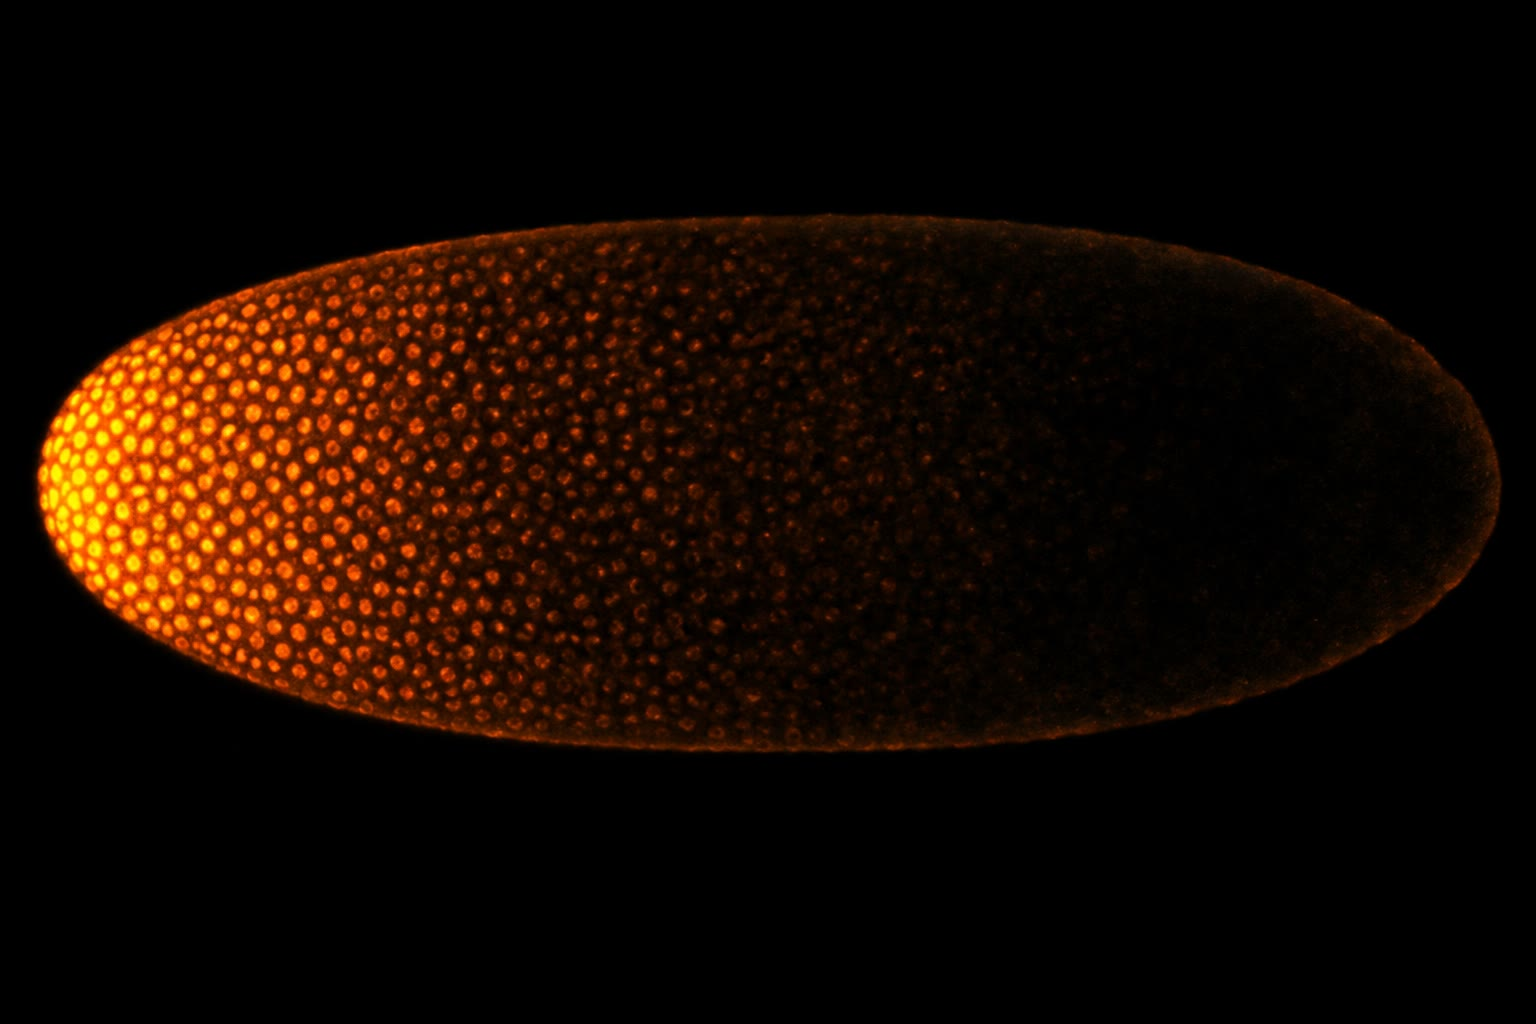
\includegraphics[width=0.46\linewidth]{images/book5/ai/b5-23-bicoid-gradient.jpg}\hspace{0.04\linewidth}
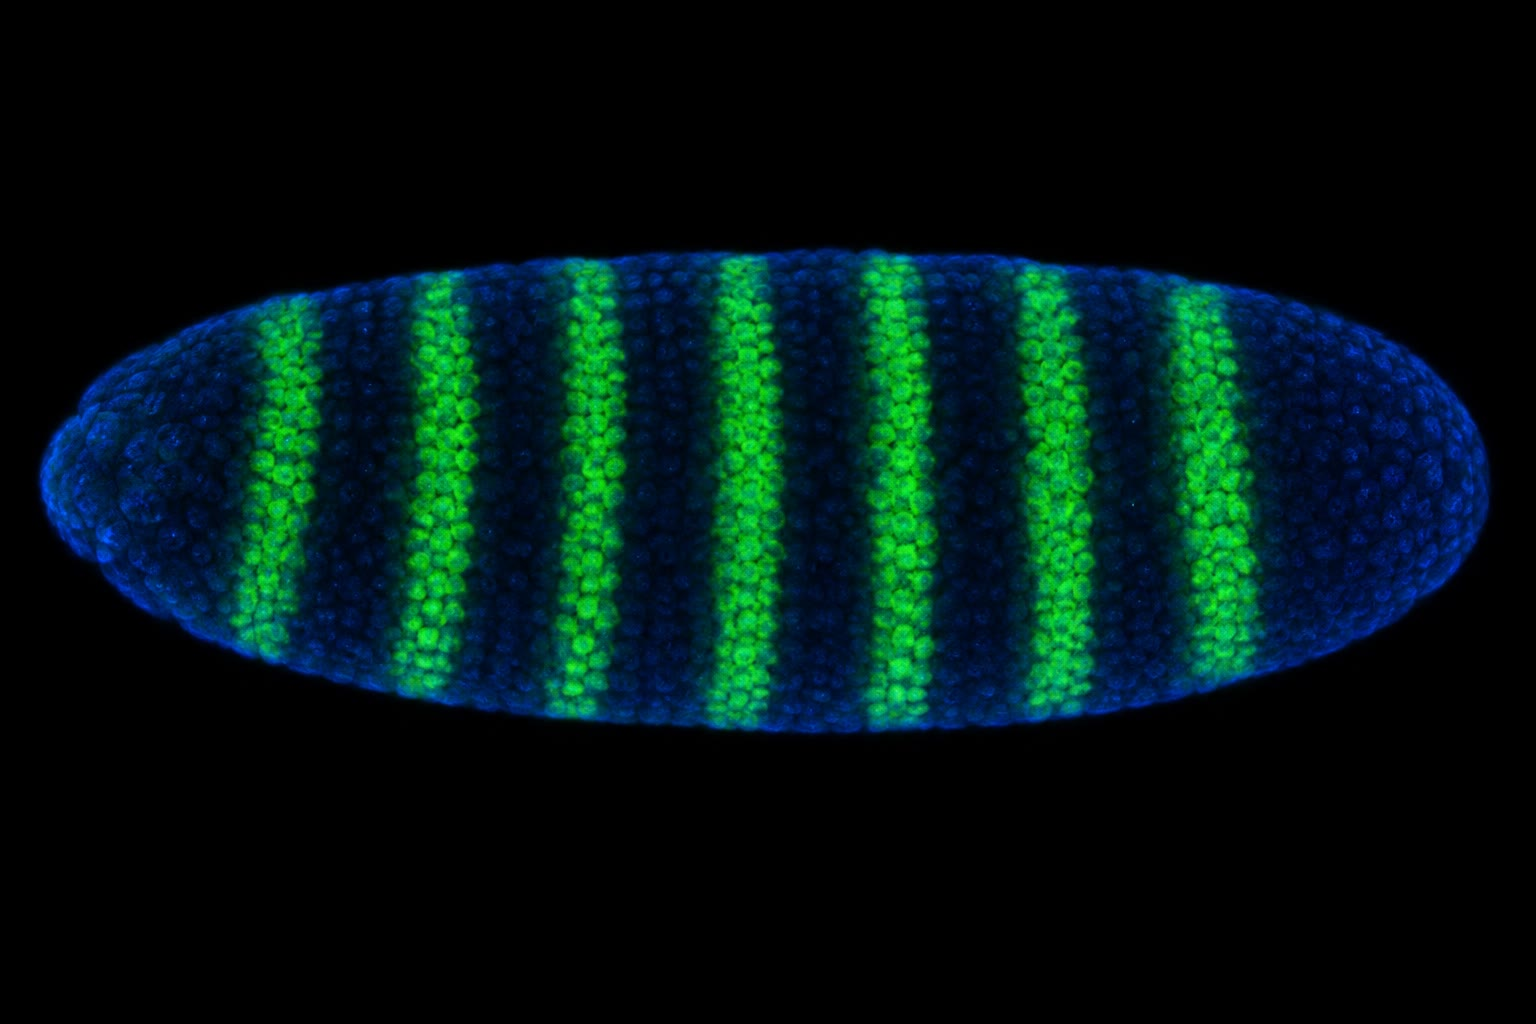
\includegraphics[width=0.46\linewidth]{images/book5/ai/b5-23-embryo-stripes.jpg}

{\small Izquierda: un embrión sincitial teñido para la proteína Bicoid,
más brillante en el polo anterior y desvaneciéndose exponencialmente
hacia el posterior. Derecha: un embrión una hora después teñido para
una proteína de regla par, con siete bandas trazadas a partir de las
bandas de los \omterm{def:b3:developmental-genetics:hierarchy}{genes gap}.}
\end{omfigure}

\section{La identidad: los genes Hox}

\begin{definition}[Genes homeóticos y colinealidad]\label{def:b3:developmental-genetics:hox}
\index{mutación homeótica}\index{genes Hox}\index{colinealidad}\index{homeobox}\index{código Hox}
Una mutación \emph{homeótica} convierte una parte del cuerpo en otra:
la palabra de Bateson (1894) para las anomalías que ``sustituyen un
miembro de una serie por otro''. En la mosca, los mutantes dominantes
de \emph{Antennapedia} desarrollan patas donde deberían ir las antenas;
los mutantes \emph{bithorax} (Lewis, 1978) convierten el tercer
segmento torácico en una copia del segundo, de modo que los
balancines (halterios) se vuelven un segundo par de alas. Los ocho
genes responsables, los \emph{genes Hox}, se sitúan en dos grupos de un
mismo cromosoma, y Lewis advirtió que su orden a lo largo del ADN
coincide con el orden a lo largo del cuerpo de los segmentos que
gobiernan ---la \emph{colinealidad}, todavía no explicada del todo.
Cada uno codifica un factor de transcripción con el mismo dominio de
unión al ADN de sesenta aminoácidos, el \emph{homeobox} (McGinnis,
Gehring, 1984), que se halló después en todos los animales: los ratones
y los seres humanos llevan cuatro grupos de trece genes cada uno,
colineales del mismo modo, expresados en dominios anidados a lo largo
del eje del cuerpo, con los genes más tardíos del grupo más
posteriores. La identidad de una célula a lo largo del eje la da la
combinación de genes Hox que expresa, el \emph{código Hox}; los genes
posteriores dominan a los anteriores (prevalencia posterior), de modo
que perder un gen posterior deja que el segmento adopte la identidad
del de delante. Los genes Hox no construyen un segmento; le dicen a un
segmento ya construido cuál es, encendiendo las baterías de genes de
más abajo que corresponden a una pata, un ala, una costilla o una
vértebra lumbar.
\end{definition}

\begin{omfigure}
\begin{tikzpicture}[every node/.style={font=\scriptsize}, >=stealth]
  % fly cluster
  \node[left] at (-0.3,2.2) {mosca (\emph{Drosophila}), 8 genes};
  \foreach \i/\g/\c in {0/lab/omDef, 1/pb/omDef, 2/Dfd/omThm, 3/Scr/omThm, 4/Antp/omMeth, 5/Ubx/omMeth, 6/abd-A/omProp, 7/Abd-B/omProp} {
    \draw[thick, fill=\c!40] ({\i*1.1},1.9) rectangle ({\i*1.1+0.9},2.5); \node[font=\tiny] at ({\i*1.1+0.45},2.2) {\emph{\g}};
  }
  \node[left] at (-0.3,0.9) {grupo HoxB del ratón, 9 de 13};
  \foreach \i/\g/\c in {0/b1/omDef, 1/b2/omDef, 2/b3/omDef, 3/b4/omThm, 4/b5/omThm, 5/b6/omMeth, 6/b7/omMeth, 7/b8/omProp, 8/b9/omProp} {
    \draw[thick, fill=\c!40] ({\i*1.1},0.6) rectangle ({\i*1.1+0.9},1.2); \node[font=\tiny] at ({\i*1.1+0.45},0.9) {\emph{\g}};
  }
  \draw[->, thick] (0,1.55) -- (9.8,1.55); \node[above, font=\tiny] at (4.9,2.55) {3$'$ $\to$ 5$'$ a lo largo del ADN};
  \draw[->, thick] (0,0.2) -- (9.8,0.2); \node[below, font=\tiny] at (4.9,0.05) {anterior $\to$ posterior a lo largo del cuerpo};
  % body schematic
  \node[left] at (-0.3,-0.9) {expresados en};
  \draw[thick, gray!70, rounded corners=6pt] (0,-1.3) rectangle (9.8,-0.5);
  \foreach \x/\t in {0.6/cabeza, 2.6/cuello, 4.4/tórax, 6.6/lumbar, 8.6/{sacro, cola}} { \node[font=\tiny] at (\x,-0.9) {\t}; }
  \draw[gray!70] (1.6,-1.3) -- (1.6,-0.5); \draw[gray!70] (3.5,-1.3) -- (3.5,-0.5); \draw[gray!70] (5.6,-1.3) -- (5.6,-0.5); \draw[gray!70] (7.6,-1.3) -- (7.6,-0.5);
  \node[below, align=center, font=\tiny] at (4.9,-1.4) {colinealidad: el orden de los genes en el cromosoma es el orden de sus dominios a lo largo del cuerpo;\\los mismos grupos, el mismo orden, de la mosca al ratón ---\\heredados de un antepasado de hace 600 millones de años};
\end{tikzpicture}

{\small Los grupos Hox de una mosca y de un ratón. Los genes se sitúan
a lo largo del ADN en el orden de las regiones corporales que
especifican, en ambos animales, y los genes homólogos se reconocen por
su secuencia: un gen \emph{Hoxb6} de ratón es reconociblemente el
\emph{Antennapedia} de la mosca.}
\end{omfigure}

\begin{proof}[Evidencia]
Lewis (1978) cartografió el complejo \emph{bithorax} como una serie de
mutaciones que transformaban cada una un segmento en el de delante,
dispuestas en el cromosoma en el orden del cuerpo, y propuso que los
genes se activaban secuencialmente a lo largo del eje. McGinnis y sus
colaboradores (1984) hallaron el \omterm{def:b3:developmental-genetics:hox}{homeobox} por hibridación cruzada entre
\emph{Antennapedia} y \emph{Ultrabithorax}, y después en ranas y
ratones. La equivalencia funcional se mostró de forma directa: un gen
\emph{Hoxb6} de ratón expresado en una mosca produce el fenotipo
\emph{Antennapedia}, patas en lugar de antenas (años noventa); un ratón
sin \emph{Hoxc8} tiene una costilla de más en su primera vértebra
lumbar, pues el segmento ha tomado la identidad del de delante; y
alterar los límites de expresión de los Hox en pollo y ratón desplaza
la posición donde se forman las extremidades anteriores, y la longitud
del cuello de un cisne corresponde a un desplazamiento posterior de ese
mismo límite.
\end{proof}

\begin{omfigure}
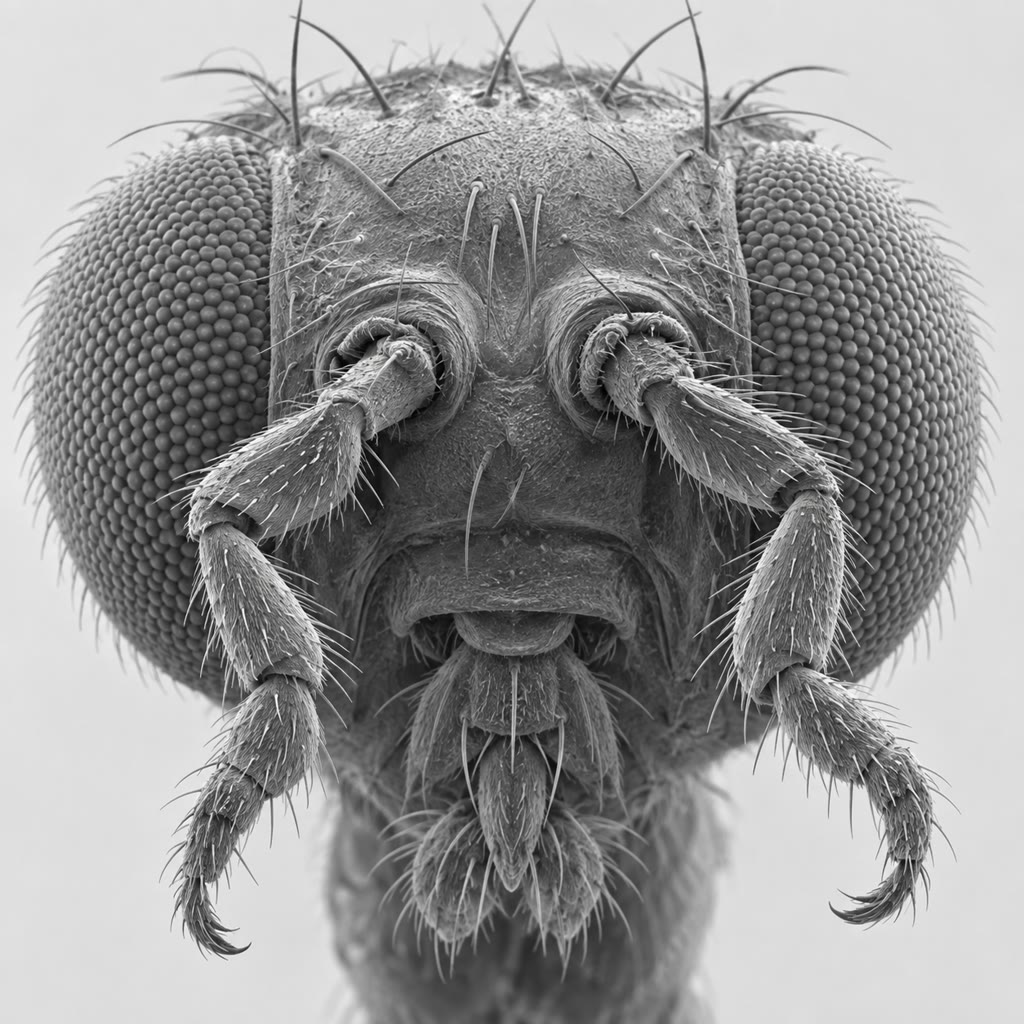
\includegraphics[width=0.34\linewidth]{images/book5/ai/b5-23-antennapedia-fly.jpg}\hspace{0.04\linewidth}
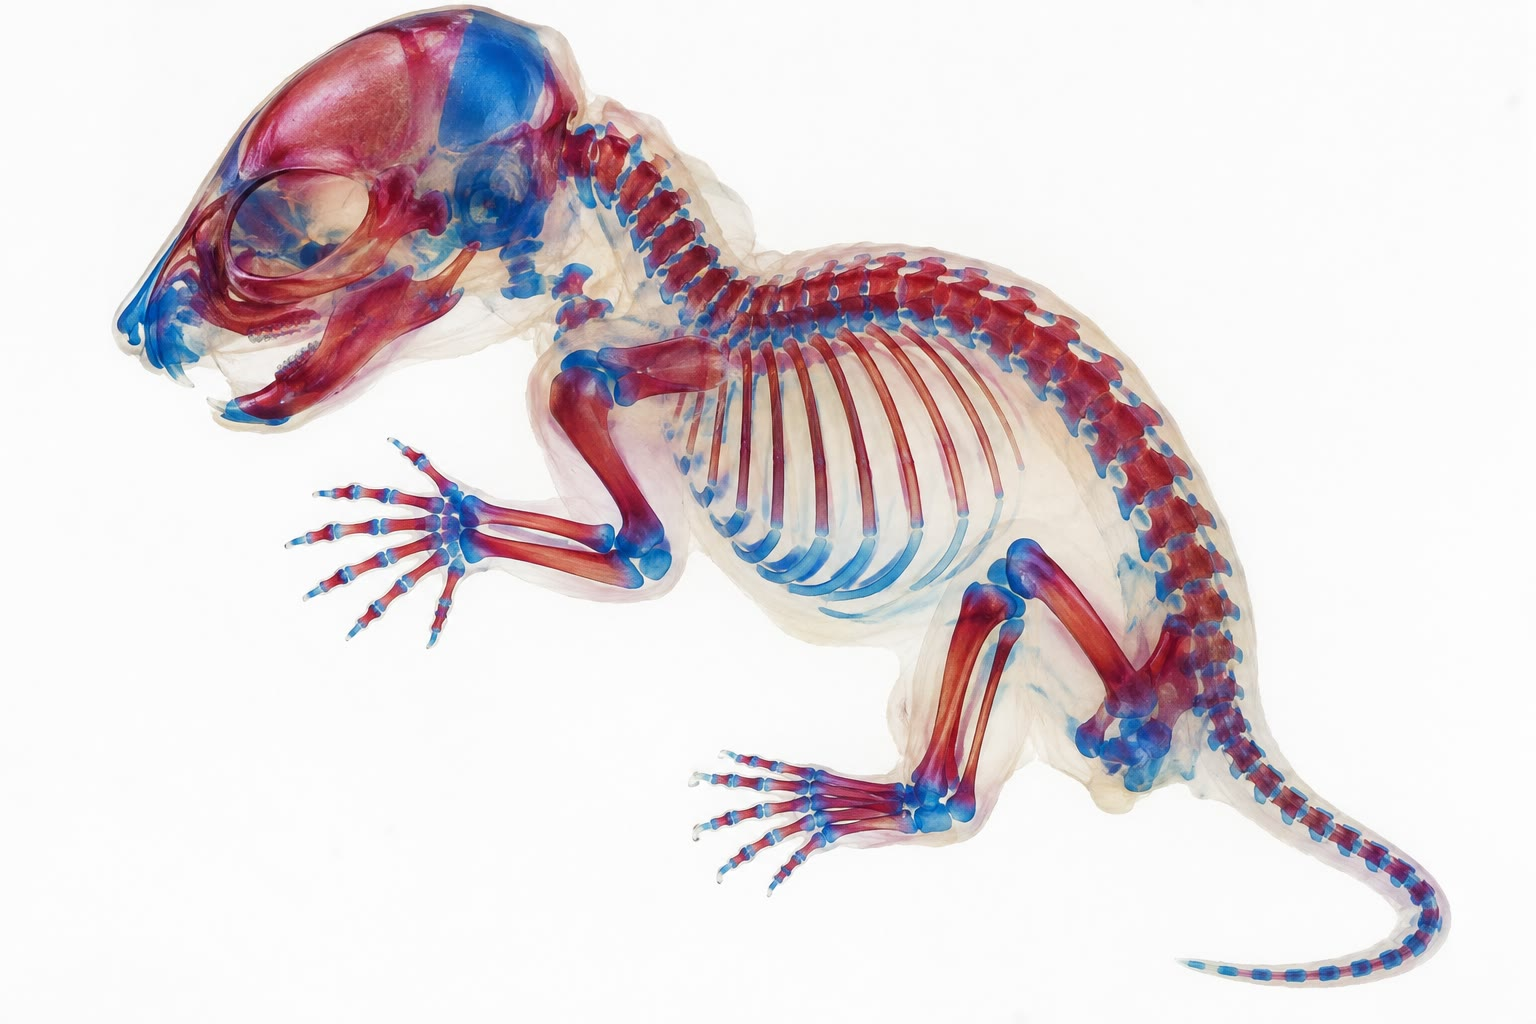
\includegraphics[width=0.5\linewidth]{images/book5/ai/b5-23-limb-skeleton-stain.jpg}

{\small Izquierda: la cabeza de una mosca mutante \emph{Antennapedia},
con un par de patas donde deberían ir las antenas ---el segmento
construido correctamente y con la identidad equivocada. Derecha: el
esqueleto de un embrión de ratón, con el cartílago en azul y el hueso
en rojo, y las vértebras a lo largo de las cuales se lee el \omterm{def:b3:developmental-genetics:hox}{código Hox}.}
\end{omfigure}

\section{Construir un vertebrado}

\begin{definition}[Organizadores y centros de señalización]\label{def:b3:developmental-genetics:organiser}
\index{organizador}\index{inducción}\index{sonic hedgehog}\index{esbozo de la extremidad}\index{zona de actividad polarizante}\index{cresta ectodérmica apical}
Los embriones de vertebrado son celulares desde el principio, de modo
que sus gradientes los hacen proteínas secretadas y no la difusión en
un sincitio, y las mismas pocas familias lo hacen todo: Wnt, Hedgehog,
BMP y otros parientes del TGF-$\beta$, FGF, Notch y el ácido retinoico.
Spemann y Mangold (1924) injertaron un trozo del labio dorsal de una
gástrula de tritón en el vientre de otra y obtuvieron un segundo
embrión, de la cabeza a la cola, hecho sobre todo de células del
huésped: el injerto era un \emph{organizador}, que inducía a sus
vecinas a formar un sistema nervioso y un eje, y setenta años más tarde
se halló que sus moléculas eran antagonistas secretados (cordina,
noguina) que bloquean la BMP, cuya ausencia deja que el ectodermo se
vuelva neural ---lo predeterminado. El \emph{tubo neural} recibe
después su patrón dorsoventral de \emph{sonic hedgehog} desde la
notocorda y la placa del suelo (alto: neuronas motoras; bajo:
\omterm{def:b3:nervous-systems:cells}{interneuronas}) frente a la BMP del techo; y el \emph{esbozo de la
extremidad}, de dos centros: la \emph{zona de actividad polarizante} de
su borde posterior, que segrega Shh (su injerto en el borde anterior da
una duplicación en espejo de los dedos, seis dedos que se encuentran
pulgar contra pulgar), y la \emph{cresta ectodérmica apical} de su
punta, que segrega FGF que mantienen en división las células
subyacentes y especifican la secuencia proximal-distal de húmero,
antebrazo y mano. El injerto, la ablación y las bolitas empapadas en
proteína siguen siendo las herramientas; la lógica ---una fuente local,
un gradiente, unos umbrales, un código de factores de transcripción---
es la de la mosca.
\end{definition}

\begin{omfigure}
\begin{tikzpicture}[every node/.style={font=\scriptsize}, >=stealth]
  % limb bud
  \fill[omDef!12] (0,0) -- (0,3) .. controls (2.6,3.4) and (3.4,2.2) .. (3.4,1.5) .. controls (3.4,0.8) and (2.6,-0.4) .. (0,0) -- cycle;
  \draw[thick, omDef] (0,0) -- (0,3) .. controls (2.6,3.4) and (3.4,2.2) .. (3.4,1.5) .. controls (3.4,0.8) and (2.6,-0.4) .. (0,0);
  \draw[very thick, omMeth!70!black] (2.9,2.5) .. controls (3.45,1.9) and (3.45,1.1) .. (2.9,0.5);
  \node[right, align=left, omMeth!70!black, font=\tiny] at (3.5,1.5) {cresta ectodérmica apical:\\FGF8; mantiene en división\\la zona de progreso;\\proximal $\to$ distal};
  \begin{scope}
    \clip (0,0) -- (0,3) .. controls (2.6,3.4) and (3.4,2.2) .. (3.4,1.5) .. controls (3.4,0.8) and (2.6,-0.4) .. (0,0) -- cycle;
    \foreach \i/\op in {1/50, 2/38, 3/26, 4/14} { \draw[omThm!\op, thick] (0.6,0.5) circle ({0.45*\i}); }
  \end{scope}
  \fill[omThm!50] (0.6,0.5) ellipse (0.5 and 0.35); \node[anchor=north, align=center, omThm, font=\tiny] at (0.9,-0.2) {ZAP: sonic hedgehog,\\posterior $\to$ anterior};
  \node[left, font=\tiny] at (-0.05,2.6) {anterior}; \node[left, font=\tiny] at (-0.05,0.4) {posterior};
  \node[left, font=\tiny] at (-0.05,1.5) {pared del cuerpo};
  \draw[->, thick] (0.3,1.5) -- (3.0,1.5); \node[above, font=\tiny] at (1.75,1.55) {húmero, antebrazo, dedos};
  % right: digit code
  \node[right, align=left] at (7.2,2.6) {identidad del dedo según la exposición a Shh:\\pulgar (dedo 1): ninguna;\\dedos 2--3: gradiente;\\dedos 4--5: de células que expresan Shh};
  \node[right, align=left] at (7.2,1.0) {injértese una segunda ZAP por delante:\\duplicación en espejo, 4-3-2-2-3-4;\\una bolita de proteína Shh hace lo mismo};
  \node[right, align=left, gray] at (7.2,-0.2) {la misma molécula da su patrón al tubo neural\\(neuronas motoras donde es alta) y al intestino};
\end{tikzpicture}

{\small Los dos centros de señalización del \omterm{def:b3:developmental-genetics:organiser}{esbozo de la extremidad}. El
\omterm{def:b3:developmental-genetics:organiser}{sonic hedgehog} del borde posterior dice a las células qué dedo ser; el
FGF de la punta les dice a qué distancia están a lo largo de la
extremidad. Los injertos que mueven un centro mueven con él el patrón.}
\end{omfigure}

\begin{proposition}[Patrón espontáneo: el mecanismo de Turing]\label{prop:b3:developmental-genetics:turing}
\index{patrón de Turing}\index{reacción--difusión}\index{activador--inhibidor}
No todo patrón se lee de un gradiente preexistente. Turing (1952)
mostró que dos sustancias que difunden y reaccionan ---un
\emph{activador} que estimula su propia producción y la de un
\emph{inhibidor}, y un inhibidor que suprime al activador y difunde
mucho más deprisa--- pueden convertir espontáneamente un campo uniforme
en una formación regular de picos: un pequeño exceso local de activador
crece por autorrefuerzo mientras el inhibidor que produce se extiende e
impide que se formen picos nuevos cerca, de modo que los picos aparecen
con un espaciado que fija el alcance del inhibidor,
$\lambda \sim \sqrt{D_{\text{inh}}/k_{\text{inh}}}$, y no coordenada
externa alguna. El mecanismo, admitido aquí en su matemática, es la
mejor explicación de las manchas y las bandas de los pelajes animales,
del espaciado de los folículos pilosos y de las yemas de las plumas, de
los pliegues del paladar, de los dedos de la mano (cuyo número sube
cuando se acorta la longitud de onda del patrón bajando la actividad
Hox) y de las bandas del pez cebra, donde se han identificado las
células que interaccionan ---células pigmentarias que repelen a las
vecinas de un tipo y atraen a distancia a las de otro--- y se ha
conseguido que sus bandas se rehagan tras una ablación con láser
exactamente como predice la teoría.
\end{proposition}
\admitted

\section{La evolución de la forma}

\begin{definition}[Evo-devo]\label{def:b3:developmental-genetics:evodevo}
\index{homología profunda}\index{caja de herramientas genética}\index{evolución cis-reguladora}\index{heterocronía}
Los genes que construyen animales son una \emph{caja de herramientas}
antigua y compartida: unos pocos cientos de factores de transcripción y
de vías de señalización presentes en el antepasado común de todos los
animales, y la diversidad animal procede sobre todo de cambios en
\emph{cuándo, dónde y cuánto} se expresan, y no en lo que codifican. La
\emph{homología profunda}: el gen \emph{Pax6} dirige la formación del
ojo en moscas, calamares y ratones, cuyos ojos no son homólogos como
órganos ---un \emph{Pax6} de ratón expresado en la pata de una mosca le
hace allí un ojo de mosca ectópico (Halder, Gehring, 1995). La
\emph{evolución cis-reguladora}: la pérdida de las espinas pélvicas en
los espinosos de agua dulce es la supresión de un solo potenciador del
gen \emph{Pitx1}, con la proteína intacta y todavía útil en otros
sitios; la pérdida de las manchas alares en algunas moscas del vinagre,
un cambio en un potenciador de \emph{yellow}; la pérdida de las patas
en las serpientes, un potenciador roto de \emph{\omterm{def:b3:developmental-genetics:organiser}{sonic hedgehog}} en la
extremidad. Los \emph{desplazamientos Hox}: el límite de expresión de
\emph{Hoxc6} marca la primera vértebra torácica por igual en ratón,
pollo, ganso y serpiente, en las vértebras 7, 14, 23 y 3; la pérdida de
las patas abdominales en los insectos fue la adquisición, por la
proteína Hox Ubx, de un dominio represor que apaga el gen de las patas
\emph{Distal-less}, allí donde en los crustáceos no lo hace. La
\emph{heterocronía}, un cambio en el momento de un programa de
desarrollo, hizo del ajolote una larva permanente y del rostro humano
el de un simio juvenil. La vieja pregunta de cómo surgen las formas
nuevas se convierte en una pregunta sobre el ADN regulador: casi todo
el genoma que importa para la forma no es gen, sino interruptor.
\end{definition}

\begin{example}[Cuatro alas]\label{ex:b3:developmental-genetics:four-wings}
Los antepasados de las moscas tenían cuatro alas, como siguen
teniéndolas las libélulas y las abejas; las moscas tienen dos, con el
par trasero reducido a los balancines. En las moscas,
\emph{Ultrabithorax} se expresa en el tercer segmento torácico y
reprime allí el programa del ala ---un centenar de genes diana, siendo
un halterio un ala con esos genes apagados. La mosca triple mutante de
Lewis, sin función de \emph{Ubx} en el tercer segmento, desarrolla un
segundo par de alas: no una estructura nueva, sino la liberación de una
antigua. En las mariposas, \emph{Ubx} se expresa también en el ala
trasera, y allí no suprime el ala, sino que cambia su patrón: la misma
proteína, otro conjunto de dianas. Cuatrocientos millones de años de
evolución de los dípteros dependieron de la decisión de un solo gen en
un solo segmento, y una sola mutación la deshace en una generación
---por lo que la historia de la forma es legible en los genes que la
construyen.
\end{example}

\begin{remark}[Geometría a partir de química]\label{rem:b3:developmental-genetics:remark}
Un embrión no tiene plano ni topógrafo. Tiene unos pocos gradientes
hechos por difusión y degradación, células que los leen frente a
umbrales y encienden factores de transcripción, y un código de esos
factores que dice a cada región en qué convertirse; tiene
\omterm{def:b3:developmental-genetics:organiser}{organizadores} locales que inducen a sus vecinos, y reacciones que se
dan su propio patrón. La matemática es la de la cinética de primer
orden y la difusión ---una exponencial, una raíz cuadrada, un umbral---
y explica no solo cómo se coloca la cabeza de una mosca, sino por qué
duplicar un gen desplaza un límite una distancia fija, por qué aparecen
seis dedos cuando se duplica una señal y por qué una serpiente tiene
trescientas costillas. La evolución edita los interruptores, no la
máquina: la caja de herramientas de una esponja y la de un ser humano
son casi la misma, y lo que difiere es el cableado.
\end{remark}

\section{Ejercicios}

\begin{exercise}[$\star$]\label{exo:b3:developmental-genetics:1}
Nómbrense los cuatro pisos de la jerarquía de segmentación de la mosca,
un gen de cada uno y el fenotipo mutante que lo colocó en su clase.
\end{exercise}

\begin{exercise}[$\star$]\label{exo:b3:developmental-genetics:2}
¿Qué es un \omterm{def:b3:developmental-genetics:hierarchy}{gen de efecto materno}? Una hembra homocigota para una
mutación nula de \emph{bicoid} se cruza con un macho silvestre:
descríbanse sus embriones y explíquese por qué su propio genotipo no
los salva.
\end{exercise}

\begin{exercise}[$\star$]\label{exo:b3:developmental-genetics:3}
Enúnciense la \omterm{def:b3:developmental-genetics:hox}{colinealidad} y la prevalencia posterior. Predígase el
fenotipo de un ratón sin \emph{Hoxc8} y el de una mosca que expresa
\emph{Antennapedia} en la cabeza.
\end{exercise}

\begin{exercise}[$\star$]\label{exo:b3:developmental-genetics:4}
¿Qué mostró el injerto de Spemann y Mangold, y qué resultaron ser las
moléculas del \omterm{def:b3:developmental-genetics:organiser}{organizador}? ¿Por qué se llama ``predeterminado'' al
destino neural?
\end{exercise}

\begin{exercise}[$\star\star$]\label{exo:b3:developmental-genetics:5}
Bicoid: $D = \qty{4}{\micro m^2/s}$, semivida \qty{35}{min}. Calcúlense
$k$, $\lambda$ y la razón de concentraciones entre el polo anterior y
el centro del huevo (\qty{250}{\micro m}).
\end{exercise}

\begin{exercise}[$\star\star$]\label{exo:b3:developmental-genetics:6}
Con $\lambda = \qty{100}{\micro m}$, un límite queda en
\qty{240}{\micro m}. ¿Dónde queda si la madre lleva cuatro copias de
\emph{bicoid} en lugar de dos? ¿Y una sola copia? Exprésense los
desplazamientos como fracción de un huevo de \qty{500}{\micro m}.
\end{exercise}

\begin{exercise}[$\star\star$]\label{exo:b3:developmental-genetics:7}
Los núcleos del blastodermo distan \qty{8}{\micro m}. Para colocar un
límite con la precisión de un núcleo con
$\lambda = \qty{100}{\micro m}$, ¿con qué precisión ha de leer un
núcleo la concentración de Bicoid? Si el núcleo cuenta moléculas
durante un tiempo $\tau$ y el recuento es de Poisson, ¿cuántas ha de
contar?
\end{exercise}

\begin{exercise}[$\star\star$]\label{exo:b3:developmental-genetics:8}
El gradiente se acerca al estado estacionario en la escala de tiempo
$1/k$. Con una semivida de \qty{35}{min}, ¿qué fracción de la
concentración estacionaria se alcanza a los \qty{60}{min}, los
\qty{90}{min} y los \qty{120}{min}? ¿Qué implica esto para un embrión
que ha de leer el gradiente antes de los \qty{150}{min}?
\end{exercise}

\begin{exercise}[$\star\star$]\label{exo:b3:developmental-genetics:9}
Se injerta una ZAP en el borde anterior del esbozo de una extremidad de
pollo. Predígase el patrón de los dedos, y el patrón si en su lugar se
implanta allí una bolita que libera una dosis baja de Shh.
\end{exercise}

\begin{exercise}[$\star\star\star$]\label{exo:b3:developmental-genetics:10}
Un morfógeno se fabrica por todo un tejido de longitud $L$ a un ritmo
$s$ por unidad de volumen, se degrada a un ritmo $k$ y se destruye en
el límite $x =
L$ (un sumidero absorbente), sin flujo en $x = 0$. Resuélvase $Dc'' - kc + s =
0$ para $c(x)$ y dibújese. ¿En qué se diferencia la forma de este
gradiente de la del caso con la fuente en un extremo, y qué ocurre
cuando $L \ll \lambda$?
\end{exercise}

\begin{exercise}[$\star\star\star$]\label{exo:b3:developmental-genetics:11}
Dos umbrales en $T_{1} = 0.3c_{0}$ y $T_{2} = 0.08c_{0}$ dividen un
gradiente en tres regiones. Muéstrese que las anchuras de las dos
primeras regiones no dependen de $c_{0}$, y explíquese por qué un
embrión cuya \emph{longitud} varía entre individuos (de \qty{450}{} a
\qty{550}{\micro m}) necesita algo más que una sola exponencial para
escalar su patrón. Propóngase un mecanismo.
\end{exercise}

\begin{exercise}[$\star\star\star$]\label{exo:b3:developmental-genetics:12}
Los espinosos perdieron las espinas pélvicas suprimiendo un potenciador
de \emph{Pitx1}, y las serpientes perdieron las extremidades rompiendo
un potenciador de \emph{\omterm{def:b3:developmental-genetics:organiser}{sonic hedgehog}}. Explíquese por qué los cambios
reguladores, y no los cambios codificantes, son la ruta habitual hacia
una estructura perdida o alterada, en términos de pleiotropía y de lo
que hace la misma proteína en otros sitios.
\end{exercise}

\section{Problema: la bandera francesa}

\begin{problem}[{Problema de fin de semana --- el sistema de
coordenadas de un huevo calculado a partir de una cinética de primer
orden: la longitud, la fuente y el tiempo de formación del gradiente de
Bicoid, los límites que traza y su precisión, lo que la dosis génica y
el tamaño del huevo les hacen, y el código Hox leído más abajo, para
terminar en la longitud de decaimiento, el desplazamiento por
duplicación y la precisión posicional}]
\label{pb:b3:developmental-genetics:1}
Datos: longitud del huevo \qty{500}{\micro m}; Bicoid, con
$D = \qty{4}{\micro m^2/s}$ y semivida \qty{35}{min}; flujo de la
fuente tal que $c_{0} = \qty{50}{nM}$ con dos copias maternas;
espaciado nuclear \qty{8.5}{\micro m} en el ciclo 14; umbrales
$T_{1} = 0.3\,c_{0}$ (cabeza/tórax) y $T_{2} =
0.08\,c_{0}$ (límite de \emph{hunchback}) para el caso de dos copias.
Ruido de lectura $\delta c/c = 0.1$ para un solo núcleo. Número de
Avogadro \qty{6e23}{}; un núcleo es una esfera de radio
\qty{3}{\micro m}.

\medskip
\noindent\textbf{Parte I --- El gradiente.}
\begin{enumerate}
  \item Calcúlese $k$ a partir de la semivida, en \unit{s^{-1}}, y la
        vida media $1/k$ en minutos.
  \item Calcúlese $\lambda = \sqrt{D/k}$ en micrómetros. ¿Cuántas
        \omterm{thm:b3:developmental-genetics:gradient}{longitudes de decaimiento} mide el huevo?
  \item ¿Por qué factor cae la concentración de un polo al otro? ¿Y por
        qué factor a lo largo de un espaciado nuclear en el centro del
        huevo?
  \item Calcúlese el flujo de la fuente $J = c_{0}\sqrt{Dk}$ en
        \unit{nM\,\micro m\,s^{-1}}, y el número de moléculas que entran
        por segundo en un parche de \qty{1}{\micro m^2} del polo
        anterior.
  \item Número de moléculas de Bicoid en un núcleo del polo ($c_{0}$) y
        en uno del centro del huevo.
  \item Fracción del estado estacionario alcanzada a los \qty{60}{min}
        y a los \qty{120}{min} ($1 - \mathrm{e}^{-kt}$). ¿Es
        estacionario el gradiente cuando se trazan los límites, hacia
        los \qty{120}{min}?
\end{enumerate}

\medskip
\noindent\textbf{Parte II --- Los límites.}
\begin{enumerate}[resume]
  \item Posiciones de los dos límites, en \unit{\micro m} y como
        fracciones de la longitud del huevo.
  \item La madre tiene cuatro copias: nuevo $c_{0}$ y las dos
        posiciones. ¿Cuánto se movió cada una? ¿Y con seis copias?
  \item Una sola copia: posiciones. ¿Qué regiones crecieron y cuáles
        encogieron?
  \item Error posicional para un ruido de lectura del \qty{10}{\%}, en
        micrómetros y en espaciados nucleares.
  \item Si el error ha de ser de un núcleo, ¿qué precisión de lectura
        hace falta? Si el núcleo promedia $n$ lecturas independientes y
        el ruido cae como $1/\sqrt{n}$, ¿cuántas lecturas?
  \item Un núcleo situado en el límite de \emph{hunchback} contiene el
        número calculado en la pregunta~5. ¿Cuál es el ruido de Poisson
        $1/\sqrt{N}$ de un solo recuento instantáneo? Compárese con el
        \qty{10}{\%} y coméntese.
\end{enumerate}

\medskip
\noindent\textbf{Parte III --- Escalado y robustez.}
\begin{enumerate}[resume]
  \item Los huevos varían de \qty{450}{} a \qty{550}{\micro m}. Si
        $\lambda$ y $c_{0}$ están fijos, ¿dónde cae el límite de
        \emph{hunchback} como fracción de la longitud del huevo en cada
        caso? ¿Está escalado el patrón?
  \item Supóngase en cambio que $D$ escala como $L^{2}$ (la misma vida
        media, pero una fuente cuya extensión crece con el huevo).
        Muéstrese que $\lambda/L$ es entonces constante y el patrón
        escala. ¿Es plausible?
  \item El gen \emph{hunchback} responde a Bicoid con un \omterm{def:b3:structural-biology:allostery}{coeficiente de
        Hill} de $5$: su expresión vale $c^{5}/(c^{5} + T^{5})$. ¿A lo
        largo de cuántos micrómetros pasa la expresión del \qty{10}{\%}
        al \qty{90}{\%} en torno al límite? Compárese con un espaciado
        nuclear.
  \item Explíquese por qué una respuesta empinada afila un límite pero
        no reduce por sí sola el error posicional debido al ruido de
        concentración.
  \item La represión mutua entre \omterm{def:b3:developmental-genetics:hierarchy}{genes gap} afila y estabiliza sus
        límites. Arguméntese en una frase por qué dos genes que se
        reprimen mutuamente no pueden estar ambos encendidos en el mismo
        núcleo en estado estacionario.
  \item La temperatura eleva $D$ un \qty{2}{\%} y $k$ un \qty{6}{\%} por
        grado. Cambio de $\lambda$ por grado, y desplazamiento del
        límite para una habitación \qty{5}{\celsius} más cálida. ¿Por
        qué podrían necesitar los embriones un mecanismo compensador?
\end{enumerate}

\medskip
\noindent\textbf{Parte IV --- La identidad.}
\begin{enumerate}[resume]
  \item El \omterm{def:b3:developmental-genetics:hox}{código Hox}: con ocho \omterm{def:b3:developmental-genetics:hox}{genes Hox} de mosca, cada uno encendido o
        apagado, ¿cuántos códigos son posibles? ¿Cuántos se usan
        (catorce segmentos)? ¿Por qué reduce la prevalencia posterior el
        número efectivo?
  \item A una mosca le falta \emph{Ubx} en su tercer segmento torácico.
        ¿En qué se convierte el segmento, y por qué el resultado son
        cuatro alas y no una estructura nueva?
  \item El límite de \emph{Hoxc6} de un ratón está en la vértebra 7, y
        el de un ganso en la 23. ¿Qué predice esto sobre sus cuellos, y
        qué cambió en la evolución: el gen o su expresión?
  \item Un injerto de ZAP da los dedos 4-3-2-2-3-4. Explíquese el patrón
        a partir de dos gradientes de Shh que se encuentran en el medio.
  \item Halder y Gehring expresaron el \emph{Pax6} de ratón en la pata
        de una mosca y obtuvieron allí un ojo de mosca. ¿Qué muestra
        esto sobre el gen, y qué \emph{no} muestra sobre los ojos de las
        moscas y de los ratones?
  \item El sexto dedo: acortar la longitud de onda de Turing añade un
        dedo. Con cinco dedos a lo ancho de una placa de mano de
        \qty{2}{mm}, ¿qué cambio de longitud de onda da seis? ¿Qué
        parámetro del sistema de reacción--difusión lo produciría?
  \item Resúmase: $\lambda$ (pregunta~2), el desplazamiento del límite
        por duplicación de la fuente (pregunta~8) y el error posicional
        para un ruido del \qty{10}{\%} (pregunta~10).
\end{enumerate}
\end{problem}
